\documentclass[aspectratio=169]{beamer}
\usetheme{Madrid}

% Pakete für die deutsche Sprache
\usepackage[T1]{fontenc}
\usepackage[utf8]{inputenc}
\usepackage[ngerman]{babel}

\usepackage{graphicx}
\usepackage{listings}
\usepackage{hyperref}

% Stil für Python-Code-Listings
\lstset{
  language=C,
  basicstyle=\ttfamily\footnotesize,
  keywordstyle=\color{blue},
  commentstyle=\color{green!50!black},
  stringstyle=\color{red},
  showstringspaces=false,
  breaklines=true,
  frame=single,
  frame=none,
  captionpos=b,
}

\title{Linux Treiber Workshop}
\subtitle{Eine Einführung in die Linux Treiber Programmierung}
\author{Johannes Roith}
\date{15.09.2023}

\begin{document}

\begin{frame}
  \titlepage
\end{frame}

\begin{frame}{Agenda}
  \tableofcontents
\end{frame}

\section{Der Linux Kernel}
\begin{frame}{Der Linux Kernel}
	\begin{itemize}
		\item Abstrahierung der Hardware
		\item Zuständig für Speicherverwaltung, Prozessverwaltung, Multitasking, Lastverteilung, Sicherheitserzwingung und Eingabe/Ausgabe-Operationen
		\item Monolithischer Kernel mit nachladbaren Modulen
		\item Zugriff auf Kernelfunktionen aus Userspace über Syscalls (open, close, read, write, ...)
	\end{itemize}
\end{frame}


\section{Unterschiede zwischen Userspace und Kernel Programmierung}
\begin{frame}{Unterschiede zwischen Userspace und Kernel Programmierung}
	\centering
	\begin{tabular}{p{0.2\textwidth}|p{0.35\textwidth}|p{0.35\textwidth}}
		& \bfseries Userspace Programm & \bfseries Kernel Modul \\
		\hline
		Resourcenzugriff: & Eingeschränkter Zugriff, benötigt Berechtigungen & Uneingeschränkter Zugriff \\
		Hardwarezugriff: & Nur über Treiber möglich & Direkter Zugriff auf Hardware möglich \\
		Programm starten: & Kann einfach über User gestartet werden & Muss in den Kernel geladen werden \\
		Latenz: & Höhere Latenz (Syscalls) & Geringe Latenzen\\
	\end{tabular}
\end{frame}

\section{Linux Kernel Programmierung auf dem Raspberry Pi}
\begin{frame}[fragile]{Linux Kernel Programmierung auf dem Raspberry Pi}
	\begin{itemize}
		\item Pakete aktualisieren mit: \lstinline|sudo apt update && sudo apt upgrade -y|
		\item Kernel Headers installieren: \lstinline|sudo apt install -y raspberrypi-kernel-headers|
		\item Build Werkzeuge, wie gcc, make, ... installieren: \lstinline|sudo apt install -y build-essential|
		\item Reboot, um ggf. neuen Kernel zu laden: \lstinline|sudo reboot|
	\end{itemize}
\end{frame}

\section{Ein erstes Hello-World Kernelmodul}
\begin{frame}[fragile]{Ein erstes Hello-World Kernelmodul}
	\begin{lstlisting}
#include <linux/module.h>
#include <linux/init.h>
int __init my_init(void)
{
	printk("hello_kernel - Hello Kernel!\n");
	return 0;
}
void __exit my_exit(void)
{
	printk("hello_kernel - Goodbye Kernel!\n");
}
MODULE_LICENSE("GPL");
MODULE_AUTHOR("Johannes Roith");
MODULE_DESCRIPTION("A simple hello world LKM");
module_init(my_init);
module_exit(my_exit);
	\end{lstlisting}
\end{frame}

\section{Makefile zum Kompilieren des Moduls}
\begin{frame}[fragile]{Makefile zum Kompilieren des Moduls}
	\begin{lstlisting}
obj-m += hello_kernel.o

all:
	make -C /lib/modules/$(shell uname -r)/build M=$(PWD) modules

clean:
	make -C /lib/modules/$(shell uname -r)/build M=$(PWD) clean
	\end{lstlisting}
\end{frame}

\section{Module verwalten mit der Bash}
\begin{frame}[fragile]{Module verwalten mit der Bash}
	\begin{itemize}
		\item \lstinline|lsmod| zeigt die geladenen Module an
		\item \lstinline|dmesg| zeigt die Kernel Logs an
		\item \lstinline|insmod <modulname>| lädt das Modul <modulname> in den Kernel
		\item \lstinline|rmmod <modulname>|  entfernt das Modul <modulname> aus den Kernel
		\item \lstinline|modprobe <modulname>|  lädt das Modul <modulname> inklusive seiner Abhängigkeiten in den Kernel
		\item \lstinline|modinfo <modulname>|  gibt Informationen über das Modul <modulname> aus
	\end{itemize}
\end{frame}

\begin{frame}{Aufgabe}
	Teste das einfache Kernelmodul auf Deinem Raspberry Pi.
\end{frame}

\section{Der Device Tree}
\begin{frame}[fragile]{Der Device Tree}
	\begin{itemize}
		\item ARM/Open RISC V Systeme haben keine automatische Hardwareerkennung wie z.B. das BIOS bei x86 Systemen
		\item Der Linux Kernel benötigt Informationen, welche Geräte verfügbar sind
		\item[$\rightarrow$] Device Tree liefert diese Informationen
		\item Device Tree fasst die verfügbaren Geräte in einer Baumstruktur zusammen
		\item Die Device Tree Sourcen (dts) und Device Tree Source Includes (dtsi)  muss kompiliert werden (dtb: Device Tree Binary)
		\item Device Tree verfügbar unter /sys/firmware/devicetree/base
		\item Umwandeln in lesbare Form: \lstinline|dtc -I fs -O dts -s /sys/firmware/devicetree/base > dt.dts|
		\item Device Tree kann auch über Overlays erweitert werden $\rightarrow$ nicht der ganze Device Tree muss neu kompiliert werden, sollte ein Gerät hinzugefügt werden
	\end{itemize}
\end{frame}

\section{Device Tree Overlays}
\begin{frame}[fragile]{Device Tree Overlays}
	\begin{lstlisting}
/dts-v1/;
/plugin/;
/ {
	fragment@0 {
		target = <&i2c1>;
		__overlay__ {
			#address-cells = <1>;
			#size-cells = <0>;
			my_adc: my_adc@10 {
				compatible = "brightlight,myadc";
				reg = <0x10>;
				status = "okay";
			};
		};
	};
};
	\end{lstlisting}
	Kompilieren des Overlays mit \lstinline|dtc -@ -I dts -O dtb -o testoverlay.dtbo testoverlay.dts|
\end{frame}

\section{Das I2C Subsystem}
\begin{frame}[fragile]{Das I2C Subsystem}{Prinzipielles Vorgehen}
	\begin{itemize}
		\item Kompatibles Gerät benennen
		\item Probe und Remove Funktionen implementieren
		\item Treiberstruktur erstellen
		\item Treiber zum Kernel hinzufügen
	\end{itemize}
\end{frame}

\begin{frame}[fragile]{Das I2C Subsystem}{Kompatible Geräte benennen}
	\begin{lstlisting}
#include <linux/i2c.h>

static struct of_device_id foo_of_ids[] = {
	{
		.compatible = "brightlight,myadc",
	}, {},
};
MODULE_DEVICE_TABLE(of, foo_of_ids);

static struct i2c_device_id foo_ids[] = {
	{"my_adc", &foo_drv_data}, {},
};
MODULE_DEVICE_TABLE(i2c, foo_ids);
	\end{lstlisting}
\end{frame}

\begin{frame}[fragile]{Das I2C Subsystem}{Probe und Remove Funktionen implementieren}
	\begin{lstlisting}
static int foo_probe(struct i2c_client *client, const struct i2c_device_id *id)
{
	...
}

static void foo_remove(struct i2c_client *client)
{
	...
}

	\end{lstlisting}
\end{frame}

\begin{frame}[fragile]{Das I2C Subsystem}{Treiberstruktur erstellen}
	\begin{lstlisting}
static struct i2c_driver foo_driver = {
	.probe = foo_probe,
	.remove = foo_remove,
	.id_table = foo_ids,
	.driver = {
		.name = "foo",
		.of_match_table = foo_of_ids,
	},
};
	\end{lstlisting}
\end{frame}

\begin{frame}[fragile]{Das I2C Subsystem}{Treiberstruktur zum Kernel hinzufügen}
	\begin{lstlisting}
int __init my_init(void)
{
	return i2c_add_driver(&foo_driver);
}

void __exit my_exit(void)
{
	i2c_del_driver(&foo_driver);
}

	\end{lstlisting}
	\begin{center}
		oder
	\end{center}
	\begin{lstlisting}
module_i2c_driver(foo_driver);
	\end{lstlisting}
\end{frame}

\begin{frame}[fragile]{Das I2C Subsystem}{Nützliche Funktionen}
	\begin{itemize}
		\item \lstinline|u8 i2c_smbus_read_byte(struct i2c_client *client)| liest ein Byte vom I2C Bus
		\item \lstinline|s32 i2c_smbus_write_byte(struct i2c_client *client, u8 data)| schreibt den Wert der Variable data auf den I2C Bus
		\item \lstinline|void mdelay(int delay_ms)| Funktion wartet delay\_ms Millisekunden. Benötigter header: \lstinline|linux/delay.h|
		\item \lstinline|void i2c_set_clientdata(struct i2c_client * client, void *data)| Setzt Daten für den I2C Client. Diese können später wieder abgerufen werden
		\item \lstinline|void *i2c_get_clientdata(struct i2c_client * client)| Ruft die gespeicherten Daten des I2C Clients ab
		\item \lstinline|void *devm_kalloc(struct device *dev, size_t size, gfp_t gfp)| Allokiert size Byte an Speicher. Der Speicher ist an die Lebensdauer des Gerätes dev gebunden und wird automatisch freigegeben, sobald das Gerät nicht mehr benötigt wird. Über gfp können Allocation flags übergeben werden. Üblich ist \lstinline|GFP_KERNEL|.
	\end{itemize}
\end{frame}

\begin{frame}[fragile]{Das I2C Subsystem}{Der Raspberry Pi Pico I2C ADC}
	\begin{itemize}
		\item Raspberry Pi Pico als Testgerät für Treiberentwicklung
		\item Poti ist an ADC0 (Analog Digital Converter) angeschlossen
		\item Wert des ADCs kann über I2C ausgelesen werden
		\item Ein Lesezugriff gibt den letzen ausgelesenen ADC Wert zurück
		\item Schreibzugriffe konfigurieren das Gerät. Wird der Wert 1 geschrieben, wird der ADC alle 500ms ausgelesen, wird eine 2 geschrieben, wird der ADC einmal ausgelesen. Bei allen anderen Werten wird der ADC nicht ausgelesen
	\end{itemize}
\end{frame}

\begin{frame}[fragile]{Das I2C Subsystem}{Der Raspberry Pi Pico I2C ADC}
	\begin{columns}
		\begin{column}{0.5\textwidth}
			\begin{center}
				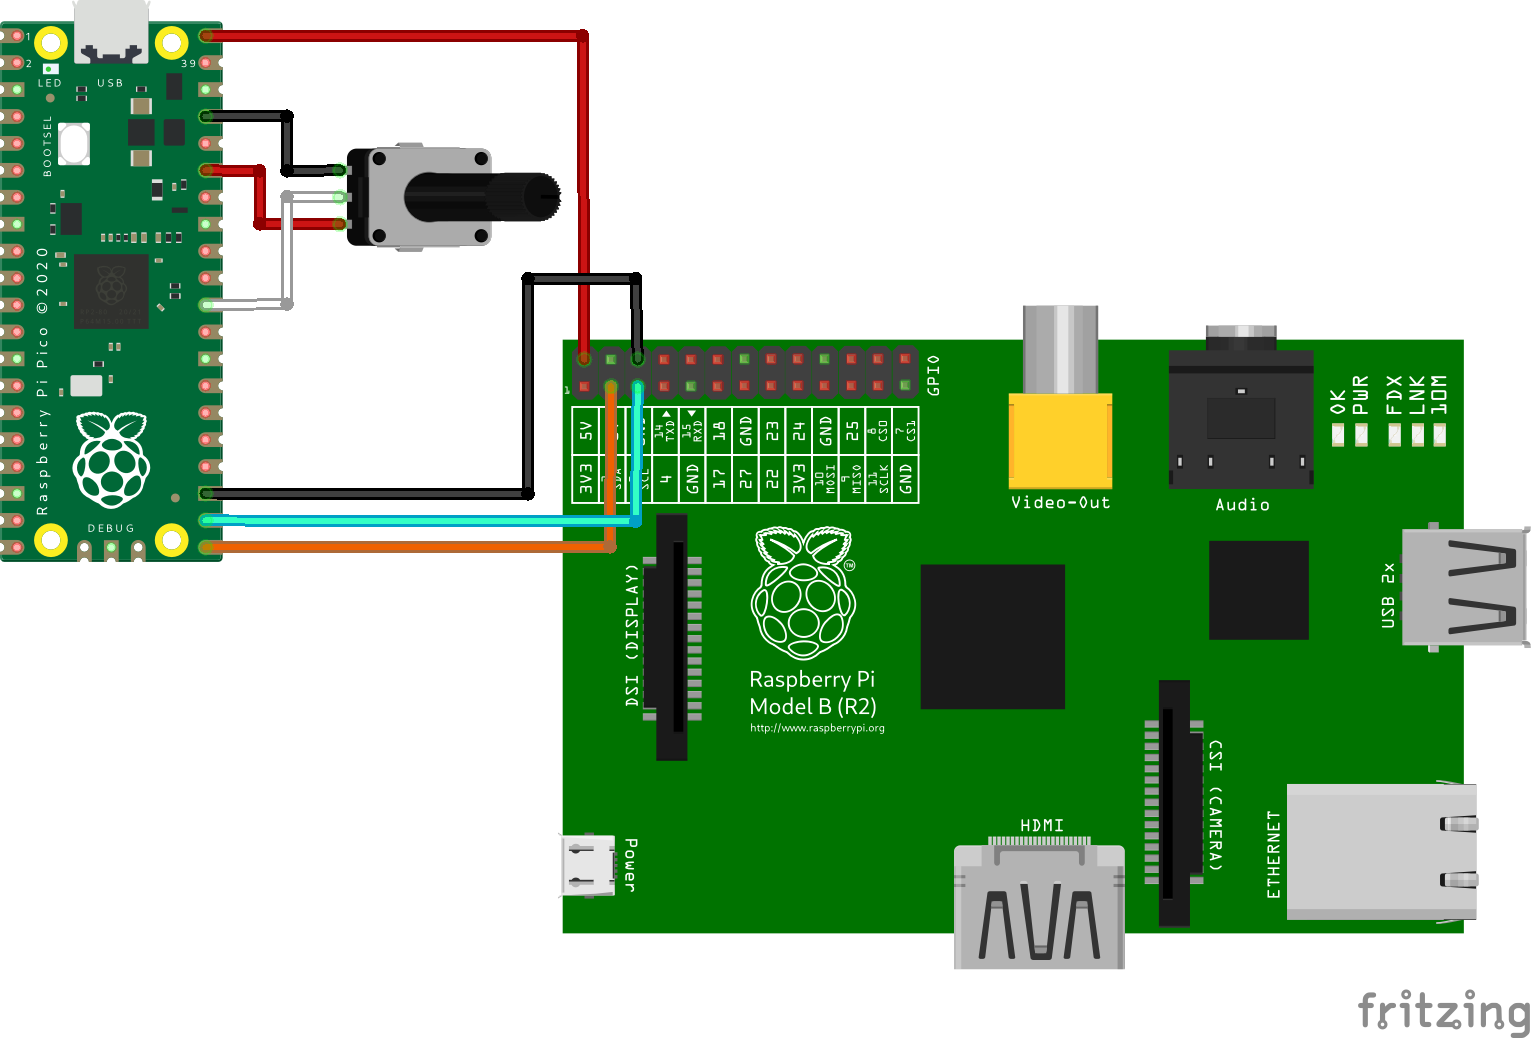
\includegraphics[width=0.95\textwidth]{Bilder/Setup_Pi_1.png}
			\end{center}
		\end{column}
		\begin{column}{0.5\textwidth}  %%<--- here
			\begin{center}
				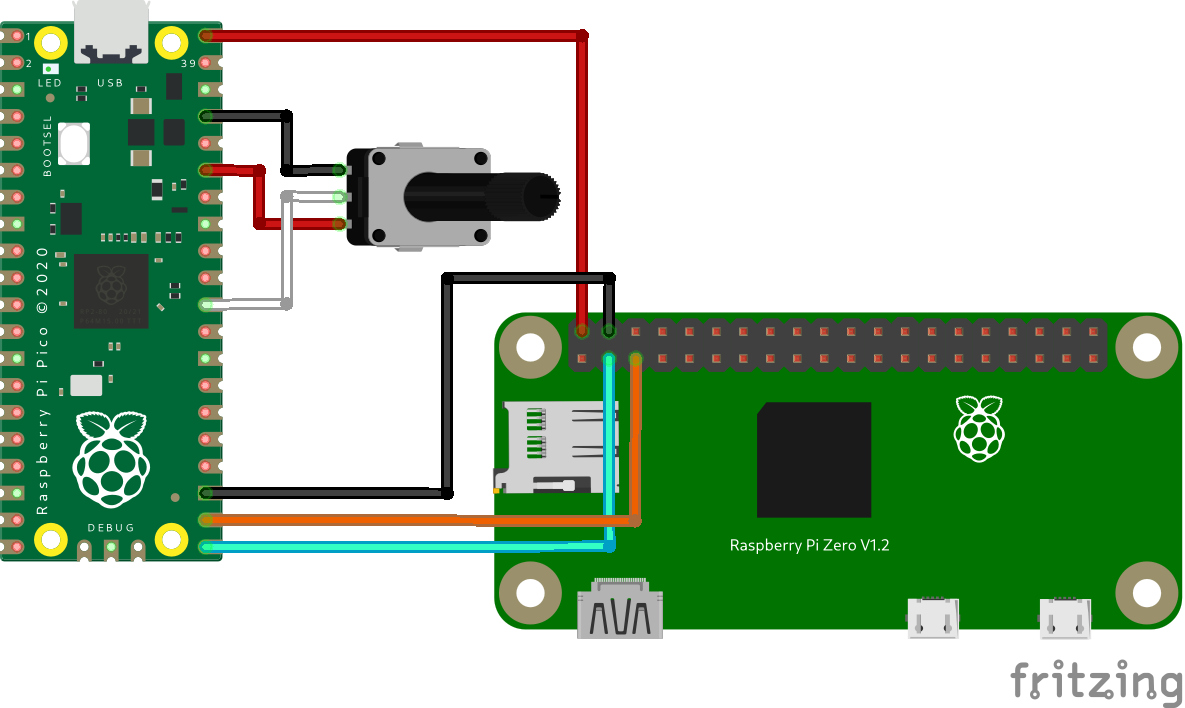
\includegraphics[width=0.95\textwidth]{Bilder/Setup_Pi_Zero.png}
			\end{center}
		\end{column}
	\end{columns}
\end{frame}

\begin{frame}[fragile]{Das I2C Subsystem}{Nützliche Shell-Befehle}
	\begin{itemize}
		\item \lstinline|i2cdetect -y 1| Scant den Bus /dev/i2c-1 nach verfügbaren Geräten ab
		\item \lstinline|i2cget -y 1 0x10| Liest ein Byte von dem I2C-Gerät mit der Adresse 0x10
		\item \lstinline|i2cset -y 1 0x10 0x12| Schreibt den Wert 0x12 zu dem I2C-Gerät mit der Adresse 0x10
	\end{itemize}
\end{frame}

\begin{frame}{Aufgaben}
	\begin{itemize}
		\item Erstelle einen Treiber für den Raspberry Pi Pico I2C ADC. in der Probe Function soll eine ADC Wandlung angestoßen, ausgelesen und das Ergebnis im Kernelog angezeigt werden 
		\item Erstelle ein Device Tree Overlay für den Raspberry Pi Pico I2C ADC
		\item Compiliere den Device Tree Overlay und lade ihn mit \lstinline|dtoverlay <overlay>|
		\item Teste Deinen Treiber
	\end{itemize}
\end{frame}

\section{Das IIO Subsystem}
\begin{frame}{Das IIO Subsystem}
	\begin{itemize}
		\item Industrial I/O
		\item Ermöglicht Zugriff auf verschiedene Sensorarten (ADCs, Temperatur-, Druck, Beschleunigungssensoren, ...)
		\item Standartisiert Schnittstelle zu verschiedenen Sensoren
		\item Zugriff über das IIO-Charaktergerät oder das IIO-Abstraktionsgerät
		\item Bietet verschiedene Funktionen zum Auslesen der Sensoren (Lesen von Rohdaten, Kalibirierung, Skalierung, ...)
	\end{itemize}
\end{frame}

\begin{frame}{Das IIO Subsystem}{Prinzipielles Vorgehen}
	\begin{itemize}
		\item Struct für IIO Gerät anlegen
		\item Read Funktion implementieren
		\item Channels und IIO Info anlegen
		\item Gerät in Probe Funktion anlegen
	\end{itemize}
\end{frame}

\begin{frame}[fragile]{Das IIO Subsystem}{Struct und Read Funktion}
	\begin{lstlisting}
#include <linux/iio/iio.h>
#include <linux/iio/sysfs.h>

struct foo {
	...
};

static int foo_read_raw(struct iio_dev * indio_dev, struct iio_chan_spec const * chan, int *val, int *val2, long mask) {
	if(mask == IIO_CHAN_INFO_RAW) {
		/* Lese Sensor aus */
		...
	} else
		return -EINVAL;
	return IIO_VAL_INT;
}
	\end{lstlisting}
\end{frame}

\begin{frame}[fragile]{Das IIO Subsystem}{Channels und IIO Info anlegen}
	\begin{lstlisting}
static const struct iio_chan_spec foo_channels[] = {
	{
		.type = IIO_VOLTAGE,
		.info_mask_separate = BIT(IIO_CHAN_INFO_RAW),
	}
};

static const struct iio_info foo_info = {
	.read_raw = foo_read_raw,
};
	\end{lstlisting}
\end{frame}

\begin{frame}[fragile]{Das IIO Subsystem}{Gerät in Probe Funktion anlegen}
	\begin{lstlisting}
int my_probe(struct i2c_client *client, const struct i2c_device_id *id)
{
	struct iio_dev *indio_dev;
	struct foo *adc;

	indio_dev = devm_iio_device_alloc(&client->dev, sizeof(struct iio_dev));
	if(!indio_dev)
		return -ENOMEM;

	adc = iio_priv(indio_dev);
	adc->client = client;
	\end{lstlisting}
\end{frame}

\begin{frame}[fragile]{Das IIO Subsystem}{Gerät in Probe Funktion anlegen}
	\begin{lstlisting}
	indio_dev->name = id->name;
	indio_dev->info = &foo_info;
	indio_dev->modes = INDIO_DIRECT_MODE;
	indio_dev->channels = foo_channels;
	indio_dev->num_channels = ARRAY_SIZE(foo_channels);

	return devm_iio_device_register(&client->dev, indio_dev);
}
	\end{lstlisting}
\end{frame}

\begin{frame}{Aufgaben}
	\begin{itemize}
		\item Erweitere den Treiber, sodass der ADC über IIO ausgelesen werden kann. Achte darauf, in Probe das Dauerhafte Auslesen des ADCs zu aktivieren (Zuerst eine 1 schreiben).
		\item Für den Treiber wird das IIO Kernelmodul benötigt. Du kannst es über \lstinline|modprobe industrialio| laden.
		\item Lese den ADC Wert über \lstinline|/sys/bus/iio/devices/iio\:device0/in_voltage_raw| aus
		\item Erweitere den Treiber, sodass in der Remove Funktion der ADC ausgeschalten wird (Schreibe eine 0 über I2C).
	\end{itemize}
\end{frame}

\end{document}
